\documentclass[11pt]{article}

\usepackage{../analysis}

\begin{document}

\coverpage{4}

% hw problem 1 -----------------------------------------------------------------

\begin{exercise}{7.3.4}{2}
    \problem{
        Suppose $f_n \to f$ and the function $f_n$ all satisfy the Lipschitz condition $| f_n(x) - f_n (y) | \leq M | x - y |$ for some constant $M$ independant of $n$.
        Prove that $f$ also satisfies the same Lipschitz condition.
    }
    \proof{
        For fixed $x,y $ in the common domain, we want to show that $| f(x) - f(y) | \leq M | x - y |$.
        Let's begin with $| f(x) - f(y) | = | f(x) - f_n (x) + f_n (x) - f_n (y) + f_n (y) - f(y) |$.
        Then by the triangle inequality applied twice, we get the following for any $n \in \N$
        $$ | f(x) - f_n (x) + f_n (x) - f_n (y) + f_n (y) - f(y) | \leq | f(x) - f_n (x)| + |f_n (x) - f_n (y) | + | f_n (y) - f(y) | $$
        By supposition, $| f_n (x) - f_n (y)| \leq M |x - y|$ so we have
        $$ | f(x) - f(y) | \leq M |x-y| + | f (x) - f_n (x) | + |f (y) - f_n (y) |$$
        for any $n$.
        But this is just a comparison of real numbers so we can just pass to the limit $n \to \infty$ and the non-strict inequality will hold.
        But the limit of the $| f - f_n | = 0$ so we have $| f(x) - f(y) | \leq M | x - y |$ as desired.
    }
\end{exercise}

% hw problem 2 -----------------------------------------------------------------

\begin{exercise}{7.3.4}{5}
    \problem{
        If $\lim _{n \to \infty} f_n = f$ and the functions $f_n$ are all monotone increasing, must $f$ be monotone increasing?
        What happens if $f_n$ are all strictly increasing?
    }
    \proof{
        In this problem, the limit $f$ must be monotone increasing.
        To see this, fix $x,y$ in the common domain $D$ such that $ x > y $.
        We know that $f_n (x) \geq f_n (y)$ for all $n \in \N$ with co-domain $\R$ so we really have a sequence of numbers satisfying
        $$ \lim _{n \to \infty} f_n (x) \geq \lim _{n \to \infty} f_n (y) $$
        When passing to the limit the non-strict inequality holds.
        By pointwise convergence of $\lim _{n \to \infty} f_n $ to $f$ we have $f(x) \geq f(y)$.
        But we just showed exactly that $f$ is monotone increasing. \parspace
        The same is not true for strictly increasing functions.
        Consider a function $f_n (x) = \frac{1}{n} x$ with domain $D = [0,1]$.
        Any $f_n$ is strictly increasing but the limit of this sequence is the function $f(x) = 0$, which is only monotone increasing.
    }
\end{exercise}

% hw problem 3 -----------------------------------------------------------------

\begin{exercise}{7.3.4}{6}
    \problem{
        Give an example of a sequence of continuous functions converging pointwise to a function with a discontinuity of the second kind.
    }
    \proof{
        We begin by defining a function with domain $[0, 1]$ and a discontinuity of the second kind at $x = 0$.
        For $x = 1/2k$, define $f(x) = 0$ and for $x = 1/(2k+1)$ define $f(x) = 1$.
        For values in between an ``even'' and ``odd'' pair, linearly interpolate between 0 and 1.
        Finally define $f(0) = 0$.
        The left figure depicts the limit (as far as I drew it).
        \begin{figure}[h]
            \centering
            \begin{tabular}{@{}*{2}{c@{}}}
                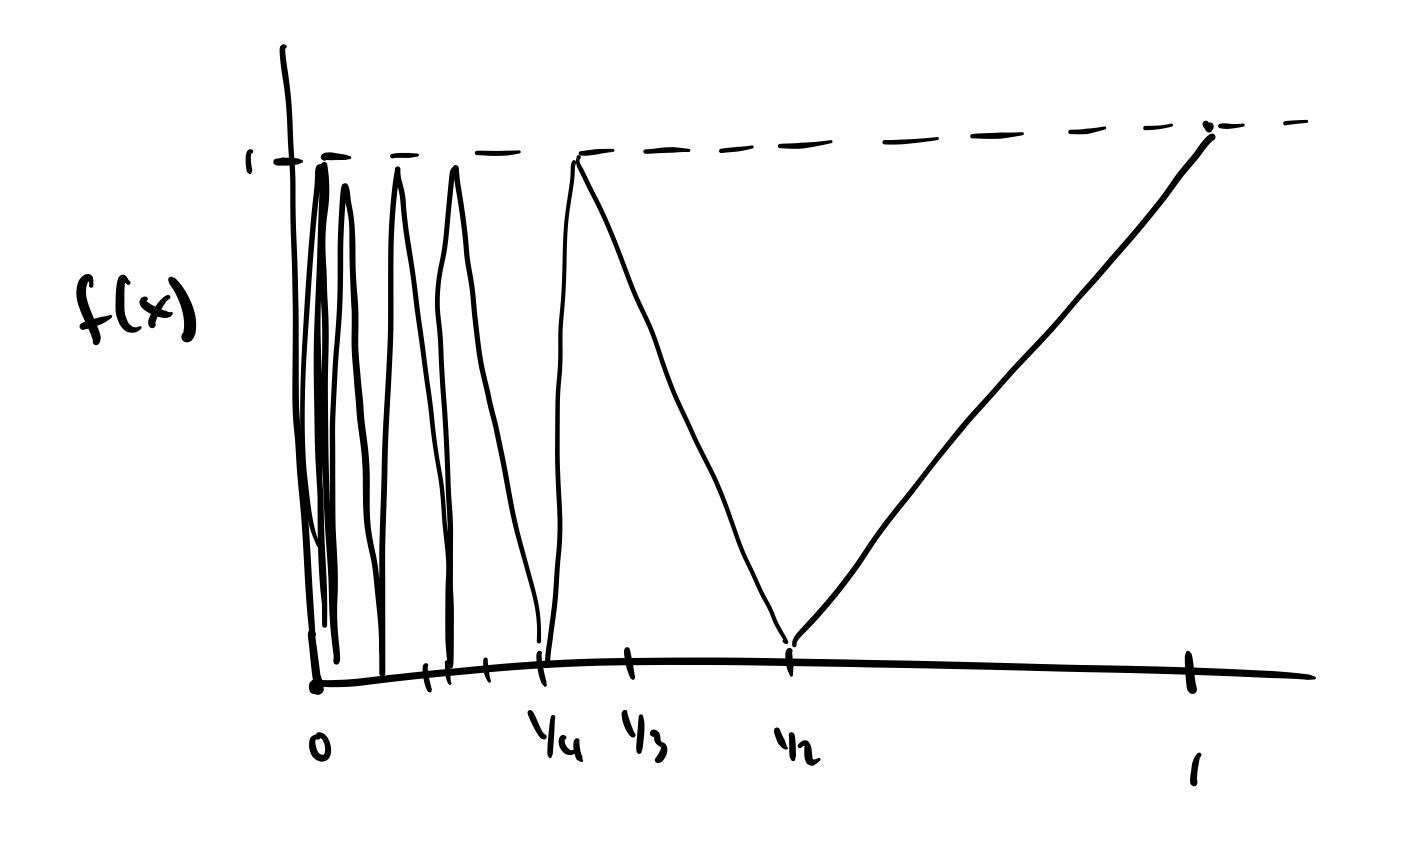
\includegraphics[width=0.4\textwidth]{img/limit}    &
                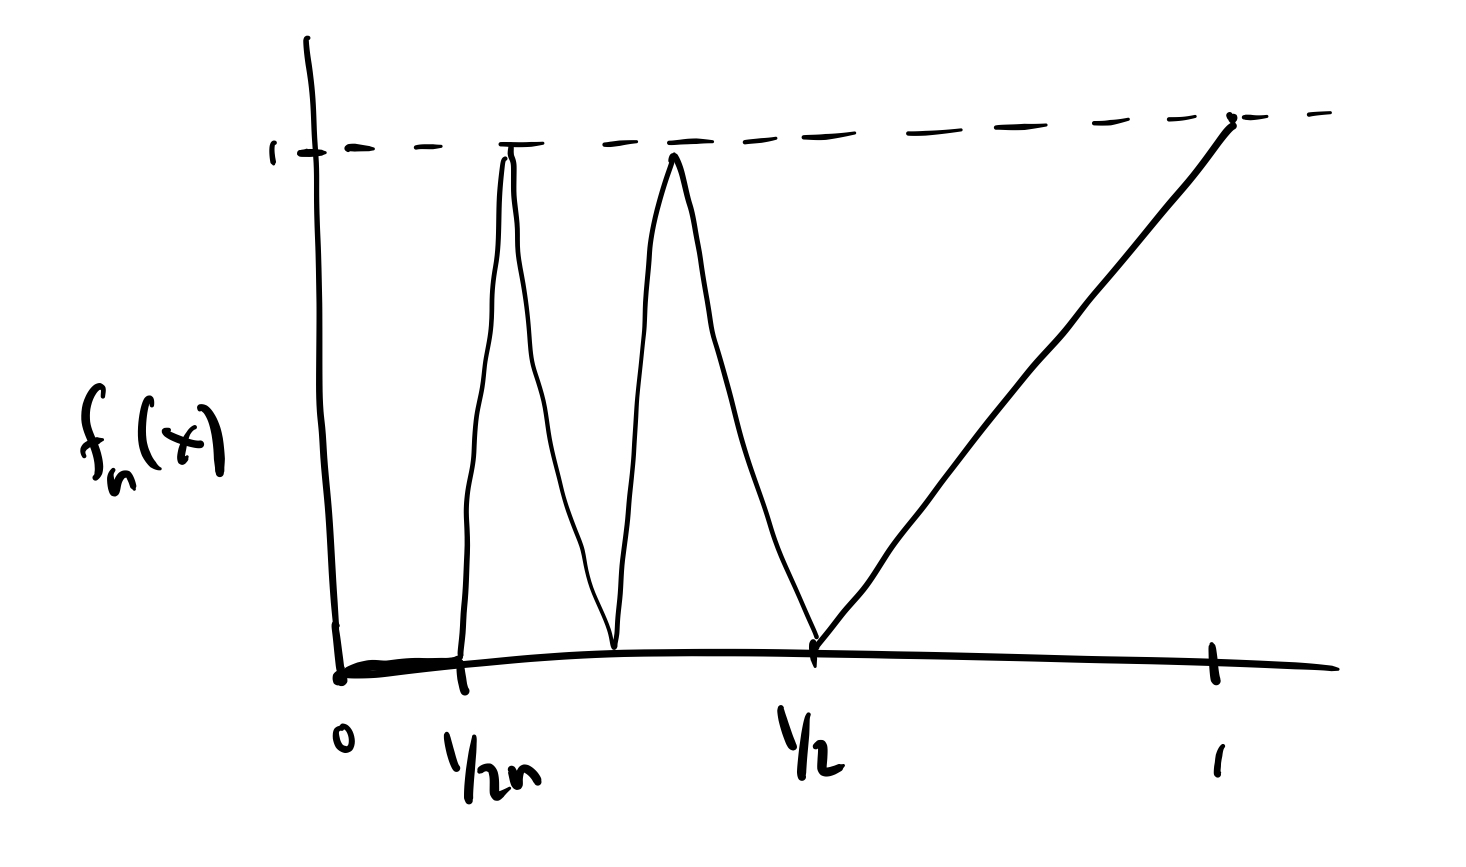
\includegraphics[width=0.4\textwidth]{img/sequence} \tabularnewline
                Limit function $f(x)$ & Element of the sequence
            \end{tabular}
            \label{fig:sequence}
        \end{figure}
        Then on the right we have a depiction of an element of the sequence.
        For a function $f_n$ in the sequence, we define $f_n (x) = 0$ for $x < 1/2n$ and defined as the limit for $x \geq 1/2n$.
        Certainly the sequence $f_1, f_2, ...$ converges pointwise to $f$ on their common domain $[0,1]$.
        Further, each $f_n$ is continuous but the limit has a discontinuity of the second kind.
    }
\end{exercise}

% hw problem 4 -----------------------------------------------------------------

\begin{exercise}{7.3.4}{7}
    \problem{
        If $| f_n (x) | \leq a_n$ for all $x$ and $\sum _{n=1}^\infty a_n$ convreges, prove that $\sum _{n=1}^\infty f_n (x)$ converges uniformly.
    }
    \proof{
        First define $F_k (x) = \sum _{n=1}^k f_n (x)$.
        Then the series $\sum _{n = 1}^\infty f_n (x)$ converges uniformly if and only if the sequence $F_1 (x), F_2 (x), ...$ has a uniform limit $F(x)$.
        By Theorem 7.3.1, the sequence $(F_k)$ has a uniform limit if and only if $(F_k)$ satisfies the Cauchy criterion: for every $1/m$ there exists some $N \in \N$ such that for all $k,j \geq N$ we have $| f_k (x) - f_j (x) | \leq 1/m$ for all $x$ in the common domain. \parspace
        Let's now show this.
        We define $A_k = \sum _{n=1}^k a_n$.
        Since the series $\sum _{n=1}^\infty a_n$ converes, we know the sequence $A_1, A_2, ...$ satisfies the Cauchy criterion for sequences of real numbers.
        Then for any $1/m$ choose $N$ such that for all $k, j \geq N$ we have $| A_k - A_j | \leq 1/m$.
        Without loss of generality, select $k \geq j$.
        Then we have
        \begin{align*}
            1/m \geq | A_k - A_j | &= | (a_1 + a_2 + \cdots + a_j + \cdots a_k) - (a_1 + a_2 + \cdots + a_k) | \\
                                   &= | a_{j+1} + \cdots + a_k | \\
                                   &\geq |\, |f_{j+1}(x)| + \cdots + |f_k (x)|\, | \\
                                   &\geq | f_{j+1}(x) + \cdots + f_k (x) | \\
                                   &= | (f_1 (x) + \cdots + f_j (x) + \cdots + f_k (x)) - (f_1 (x) + \cdots + f_j (x) | \\
                                   &= | F_k (x) - F_j (x) |
        \end{align*}
        This is exactly the Cauchy criterion for sequences of functions.
        So we have shown that $\sum _{n=1}^\infty f_n (x)$ converges uniformly. 
    }
\end{exercise}

\end{document}
